\chapter{Specifikacija programske potpore}
		
	\section{Funkcionalni zahtjevi}

			
			\noindent \textbf{Dionici:}
			
			\begin{packed_enum}
				
				\item Administrator
				\item Korisnik				
				\item Organizator				
				\item Posjetitelj
				\item Baza podataka
				\item PayPal
				\item Banka
				
				
			\end{packed_enum}
			
			\noindent \textbf{Aktori i njihovi funkcionalni zahtjevi:}
			
			
			\begin{packed_enum}
				\item  \underbar{Administrator (inicijator) može:}
				
				\begin{packed_enum}
					
					\item prijaviti se i odjaviti sa stranice
					\item pregledavati događaje
					\begin{packed_enum}
	
							\item  filtrirati događaje po vremenskom razdoblju
	
					\end{packed_enum}
					\item  upravljati korisnicima
					\begin{packed_enum}
						
							\item  urediti ili izbrisati korisničke profile
							\item  urediti ili izbrisati objave korisnika
																			
				    \end{packed_enum}
					\item  postavljati cijene članstva
					
				\end{packed_enum}
			
			 	\item  \underbar{Korisnik  (inicijator) može:}
			 	
			 	\begin{packed_enum}
			 		
			 		\item prijaviti se i odjaviti sa stranice
			 		\item napraviti profil
			 		\item prikazati profil i urediti ga
			 		\item pregledavati događaje
			 		\begin{packed_enum}
			 			
			 			\item  filtrirati događaje po vremenskom razdoblju
			 			
			 		\end{packed_enum}
			 		
			 	\end{packed_enum}
			    
			    \newpage
			    
			    \item  \underbar{Organizator (inicijator) može:}
				
				\begin{packed_enum}
					
					\item postaviti događaj
					\begin{packed_enum}
						
						\item  urediti ili izbrisati događaj
						\item  postaviti događaj sa plaćanjem ulaznice i platiti članarinu (Paypalom ili bankovnom karticom)
						
					\end{packed_enum}
					\item prijaviti se i odjaviti sa stranice
					\item napraviti profil
					\item prikazati profil i urediti ga
					\item pregledavati događaje
					\begin{packed_enum}
	
						\item filtriraj događaje po vremenskom razdoblju
	
					\end{packed_enum}
					
				\end{packed_enum}
				
				\item  \underbar{Posjetitelj   (inicijator) može:}
				
				\begin{packed_enum}
					\item iskazati interese za događaj („sigurno dolazim“, „možda dolazim“, „ne dolazim“)
					\item recenzirati događaj	
					\item prijaviti se i odjaviti sa stranice
					\item napraviti profil
					\item prikazati profil i urediti ga
					\item uključiti obavijesti o najnovijim događajima po kriterijima: vrsta događanja i područje
					\item pregledavati događaje
					\begin{packed_enum}
						
						\item  filtrirati događaje po vremenskom razdoblju
						
					\end{packed_enum}
					
				\end{packed_enum}
				
				\item  \underbar{Baza podataka (sudionik):}	
							
				\begin{packed_enum}				
				
					\item pohranjuje zapise o korisnicima i događajima
					\item pohranjuje iskazane interese za događaje
					\item pohranjuje recenzije događaja			
					\item pohranjuje informacije o cijenama članstva
					\item omogućuje prijavu i odjavu sa stranice (token)
				\end{packed_enum}

				\item  \underbar{PayPal (sudionik):}

				\begin{packed_enum}

				\item Odobrava transakcije potrebne za platiti članarinu

				\end{packed_enum}				
				
				\item  \underbar{Banka (sudionik):}				
				
				\begin{packed_enum}
						
				\item Odobrava transakcije potrebne za platiti članarinu 					
					
				\end{packed_enum}
			    
			   
					

												
			\end{packed_enum}
			
	
			\eject 
			
			
				
			\subsection{Obrasci uporabe}
							
					\noindent \underbar{\textbf{UC1 - Registracija posjetiteljskog računa}}
					\begin{packed_item}
					\item \textbf{Glavni sudionik:} Korisnik
					\item  \textbf{Cilj:} Izrada korisničkog računa za potrebe pregledavanja i posjećivanja događaja
					\item  \textbf{Sudionici:} Baza podataka
					\item  \textbf{Preduvjet:} -
					\item  \textbf{Opis osnovnog tijeka:}
					
					\item[] \begin{packed_enum}
						
						\item Korisnik izabire opciju registracije
						\item Korisnik unosi korisničke podatke koji se od njega traže
						\item Sustav provjerava ispravnost unesenih podataka te šalje obavijest potvrde registracije
						\item Sustav šalje korisnika na prozor za prijavu na stranicu
					\end{packed_enum}
					
											\item  \textbf{Opis mogućih odstupanja:}
					
					\item[] \begin{packed_item}
						
						\item[2.a] Korisnik odabire već zauzeto korisničko ime ili e-mail ili navodi neispravni e-mail
						\item[] \begin{packed_enum}
							
							\item Sustav obavještava korisnika o neuspješnoj registraciji, navodi razlog zašto
							registracija nije uspjela te ga vraća na stranicu za registraciju
							\item Korisnik promijeni potrebne podatke, završi registraciju ili odustane od registracije
							
						\end{packed_enum}
					\end{packed_item}

				\end{packed_item}
				
					\noindent \underbar{\textbf{UC2 - Registracija organizatorskog računa}}
					\begin{packed_item}
					\item \textbf{Glavni sudionik:} Korisnik
					\item  \textbf{Cilj:} Izrada korisničkog računa za potrebe stvaranja/organiziranja događaja
					\item  \textbf{Sudionici:} Baza podataka
					\item  \textbf{Preduvjet:} -
					\item  \textbf{Opis osnovnog tijeka:}
					
					\item[] \begin{packed_enum}
						
						\item Korisnik izabire opciju registracije uz odabir polja "Organizator"
						\item Korisnik unosi korisničke podatke
						\item Sustav provjerava ispravnost unesenih podataka te šalje obavijest potvrde registracije
						\item Sustav šalje korisnika na prozor za prijavu na stranicu
					\end{packed_enum}
					
											\item  \textbf{Opis mogućih odstupanja:}
					
					\item[] \begin{packed_item}
						
						\item[2.a] Korisnik odabire već zauzeto korisničko ime ili e-mail, ili unosi neispravne podatke u ostalim poljima 
						\item[] \begin{packed_enum}
							
							\item Sustav obavještava korisnika o neuspješnoj registraciji, navodi razlog zašto
							registracija nije uspjela te ga vraća na stranicu za registraciju
							\item Korisnik promijeni potrebne podatke, završi registraciju ili odustane od registracije
							
						\end{packed_enum}
					\end{packed_item}
					
				\end{packed_item}
			
					\noindent \underbar{\textbf{UC3 - Prijava na stranicu}}
					\begin{packed_item}
				
				\item \textbf{Glavni sudionik: } Korisnik, Administrator
				\item  \textbf{Cilj:} Dobiti pristup stranici
				\item  \textbf{Sudionici:} Baza podataka
				\item  \textbf{Preduvjet:} Korisnik ima registrirani račun ili ima račun s pravima administratora
				\item  \textbf{Opis osnovnog tijeka:}
				
				\item[] \begin{packed_enum}
					
					\item Korisnik/Administrator otvara stranicu
					\item Korisnik/Administrator unosi korisničke podatke za prijavu na stranicu
					\item Sustav prepoznaje je li prijavljeni račun korisnički ili administratorski, daje obavijest o uspješnoj prijavi te otvara odgovarajuću početnu stranicu
				\end{packed_enum}
				
				\item  \textbf{Opis mogućih odstupanja:}
				
				\item[] \begin{packed_item}
					
					\item[2.a] Korisnik unosi pogrešnu kombinaciju imena i lozinke za prijavu
					\item[] \begin{packed_enum}
						
						\item Sustav javlja korisniku da je prijava neuspješna, nudi ponovnu prijavu ili stvaranje
						novog korisničkog računa
					\end{packed_enum}
					
					
				\end{packed_item}
			\end{packed_item}
			
				
					\noindent \underbar{\textbf{UC4 - Pregled događaja}}
					\begin{packed_item}
					\item \textbf{Glavni sudionik:} Korisnik
					\item  \textbf{Cilj:} Pregledati dostupne događaje
					\item  \textbf{Sudionici:} Baza podataka
					\item  \textbf{Preduvjet:} Korisnik se prijavio na stranicu
					\item  \textbf{Opis osnovnog tijeka:}
					
					\item[] \begin{packed_enum}
						
						\item Nakon prijave korisnika se prebacuje na stranicu za pregledavanje događaja
						\item Korisniku su događaji izlistani jedan ispod drugog
						\item Kod svakog događaja prikazane su sve informacije o događaju (npr. datum održavanja, broj zainteresiranih itd.)te pripadajuća fotografija
					\end{packed_enum}
					
				\end{packed_item}
				
					\noindent \underbar{\textbf{UC5 - Filtriranje događaja}}
					\begin{packed_item}
					\item \textbf{Glavni sudionik:} Korisnik
					\item  \textbf{Cilj:} Pregledati događaje prema željenim kriterijima
					\item  \textbf{Sudionici:} Baza podataka
					\item  \textbf{Preduvjet:} Korisnik je prijavljen i nalazi se na stranici za pregled događaja
					\item  \textbf{Opis osnovnog tijeka:}
					
					\item[] \begin{packed_enum}
						
						\item Korisnik na stranici za pregledavanje događaja bira između više ponuđenih opcija za sortiranje događaja
					\end{packed_enum}
					
					\item  \textbf{Opis mogućih odstupanja:}
					
					\item[] \begin{packed_item}
						
						\item[1.a] Ne postoji događaj koji odgovara korisnikovoj kombinaciji filtera
						\item[] \begin{packed_enum}
							
							\item Sustav korisniku javlja da ne postoji događaj koji odgovara njegovoj kombinacijom filtera
							
						\end{packed_enum}
					\end{packed_item}
				\end{packed_item}

					\noindent \underbar{\textbf{UC6 - Prikazivanje osobnog profila}}
					\begin{packed_item}
					\item \textbf{Glavni sudionik:} Korisnik 
				\item  \textbf{Cilj:} Pregledati osobni profil
				\item  \textbf{Sudionici:} Baza podataka
				\item  \textbf{Preduvjet:} Korisnik je prijavljen na stranici
				\item  \textbf{Opis osnovnog tijeka:}
	
				\item[] \begin{packed_enum}
		
				\item Korisnik odabire opciju "Profil"
				\item Stranica prikazuje korisnikov osobni profil
				\end{packed_enum}
	
			\end{packed_item}

					\noindent \underbar{\textbf{UC7 - Uređivanje profila}}
					\begin{packed_item}
	\item \textbf{Glavni sudionik:} Korisnik
	\item  \textbf{Cilj:} Izmjena osobnih podataka
	\item  \textbf{Sudionici:} Baza podataka
	\item  \textbf{Preduvjet:} Korisnik je prijavljen na stranici i odabrao je opciju "Profil" (UC6)
	\item  \textbf{Opis osnovnog tijeka:}
	
	\item[] \begin{packed_enum}
		
		\item Korisnik na stranici osobnog profila odabire opciju "Uredi profil"
		\item Sustav korisniku otvara stranicu na kojoj može promijeniti osobne podatke
		\item Korisnik mijenja jedan ili više osobnih podataka
		\item Korisnik odabire opciju "Spremi promjene"
		\item Sustav korisniku javlja da su promjene uspješno pohranjene te ga vraća na stranicu profila
	\end{packed_enum}
	
	\item  \textbf{Opis mogućih odstupanja:}
	
	\item[] \begin{packed_item}
		
		\item[4.a] Korisnik je promijenio korisničko ime u nešto što već postoji u sustavu
		\item[] \begin{packed_enum}
			
			\item Sustav javlja korisniku da je novo korisničko ime zauzeto
			\item Korisnik ponovno upisuje korisničko ime ili odustaje od promjena te odabire opciju "Odustani"
			
		\end{packed_enum}
	\end{packed_item}
\end{packed_item}

					\noindent \underbar{\textbf{UC8 - Odjava sa stranice}}
					\begin{packed_item}
	\item \textbf{Glavni sudionik:} Korisnik, Administrator
	\item  \textbf{Cilj:} Odjaviti se sa stranice
	\item  \textbf{Sudionici:} Baza podataka
	\item  \textbf{Preduvjet:} Korisnik/Administrator je prijavljen na stranici
	\item  \textbf{Opis osnovnog tijeka:}
	
	\item[] \begin{packed_enum}
		
		\item Korisnik/Administrator odabire opciju "Odjava"
		\item Sustav odjavljuje korisnika/administratora sa stranice
	\end{packed_enum}

\end{packed_item}

					\noindent \underbar{\textbf{UC9 - Izražavanje interesa}}
\begin{packed_item}
	\item \textbf{Glavni sudionik:} Posjetitelj
	\item  \textbf{Cilj:} Izraziti interes za neki ponuđeni događaj
	\item  \textbf{Sudionici:} Baza podataka
	\item  \textbf{Preduvjet:} Korisnik je prijavljen na stranici i njegov račun je posjetiteljski
	\item  \textbf{Opis osnovnog tijeka:} 
	
	\item[] \begin{packed_enum}
		
		\item Posjetitelj pregledava događaje (UC4) te dolazi do događaja koji ga zanima
		\item Posjetitelj odabire opciju "Moj interes" 
		\item Posjetitelju se otvara obrazac za izražavanje interesa gdje mu se nude tri opcije: "sigurno dolazim", "možda dolazim", "ne dolazim"
		\item Posjetitelj odabire jednu od ponuđenih opcija
		\item Sustav pohranjuje podatak o posjetiteljevom interesu i u slučaju da je posjetitelj odabrao "sigurno dolazim" ili "možda dolazim" ažurira odgovarajući brojač kod prikaza događaja
	\end{packed_enum}
	
		\item  \textbf{Opis mogućih odstupanja:}
	
	\item[] \begin{packed_item}
		
		\item[2] Posjetitelj odabrao opciju "Moj interes", no nije odabrao niti jednu ponuđenu opciju
		\item[] \begin{packed_enum}
			
			\item Sustav ne ažurira brojač i ne događa se nikakva promjena kod prikaza događaja
			
		\end{packed_enum}
		\item[4] Posjetitelj odabrao pogrešnu opciju ili želi promijeniti interes
		\item[] \begin{packed_enum}
			
			\item Posjetitelj ponovno odabire opciju "Moj interes" i odabire drugu opciju
			
		\end{packed_enum}
		
	\end{packed_item}

\end{packed_item}


					\noindent \underbar{\textbf{UC10 - Pregled posjetiteljevih interesnih događaja}}
\begin{packed_item}
	\item \textbf{Glavni sudionik:} Posjetitelj
	\item  \textbf{Cilj:} Pregledati sve događaje koje posjetitelja zanimaju
	\item  \textbf{Sudionici:} Baza podataka
	\item  \textbf{Preduvjet:} Posjetitelj je prijavljen i na početnoj je stranici
	\item  \textbf{Opis osnovnog tijeka:}
	
	\item[] \begin{packed_enum}
		
		\item Posjetitelj na početnoj stranici odabire opciju "Pregled interesnih događaja"
		\item Sustav posjetitelju otvara stranicu na kojoj je popis svih događaja za koje je postavio interes "sigurno dolazim" ili "možda dolazim"
	\end{packed_enum}
	
	\item  \textbf{Opis mogućih odstupanja:}
	
	\item[] \begin{packed_item}
		
		\item[2.a] Posjetitelj nije odabrao odgovarajuću opciju niti za jedan događaj
		\item[] \begin{packed_enum}
			
			\item Sustav korisniku porukom javlja kako nema događaja za prikaz
			
		\end{packed_enum}
	\end{packed_item}
\end{packed_item}

					\noindent \underbar{\textbf{UC11 - Recenziranje događaja}}
\begin{packed_item}
	\item \textbf{Glavni sudionik:} Posjetitelj
	\item  \textbf{Cilj:} Ostaviti recenziju na posjećen događaj
	\item  \textbf{Sudionici:} Baza podataka
	\item  \textbf{Preduvjet:} Posjetitelj je prijavljen na stranicu i nalazi se na stranici pregleda interesnih događaja (UC10)
	\item  \textbf{Opis osnovnog tijeka:}
	
	\item[] \begin{packed_enum}
		
		\item Posjetitelj dolazi do događaja kojeg želi recenzirati i odabire opciju "Recenziraj!"
		\item Ako je događaj završio i nije prošlo 48 sati od njegovog završetka, posjetitelju se otvara obrazac za recenziranje u kojem posjetitelj odabire ocjenu te piše recenziju
		\item Posjetitelj završava recenziju i odabire opciju "Spremi recenziju"
		\item Sustav pohranjuje recenziju te javlja posjetitelju da je recenzija uspješna
		\item Ako događaj nije završio, ili je prošlo više od 48 sati od njegovog završetka, sustav javlja posjetitelju kako nije moguće ostaviti recenziju i navodi razlog
	\end{packed_enum}
			\item[2.a] Posjetitelj ostavio ocjenu, no nije ostavio opis recenzije
	\item[] \begin{packed_enum}
		
		\item Sustav javlja posjetitelju da mora napisati opis
		\item Posjetitelj piše opis i sprema recenziju, ili odustaje odabirom opcije "Odustani"
		
	\end{packed_enum}
	
\end{packed_item}

					\noindent \underbar{\textbf{UC12 - Automatsko slanje obavijesti}}
\begin{packed_item}
	\item \textbf{Glavni sudionik:} Posjetitelj
	\item  \textbf{Cilj:} Kroz aplikaciju postaviti automatsko primanje obavijesti za najnovije događaje na temelju zadanih kriterija
	\item  \textbf{Sudionici:} Baza podataka
	\item  \textbf{Preduvjet:} Posjetitelj prijavljen i nalazi se na stranicu osobnog korisničkog računa
	\item  \textbf{Opis osnovnog tijeka:}
	
	\item[] \begin{packed_enum}
		
		\item Korisnik odabire opciju "Uključi obavijesti o novim događajima"
		\item Korisnik zadaje kriterij: vrstu događaja te područje
		\item Korisnik odabire opciju "Spremi" te sustav pohranjuje korisnikov odabir
	\end{packed_enum}

\end{packed_item}



					\noindent \underbar{\textbf{UC13 - Postavljanje događaja}}
\begin{packed_item}
	\item \textbf{Glavni sudionik:} Organizator
	\item  \textbf{Cilj:} Postaviti novi događaj
	\item  \textbf{Sudionici:} Baza podataka
	\item  \textbf{Preduvjet:} Korisnik je prijavljen na stranici i ima organizatorski račun
	\item  \textbf{Opis osnovnog tijeka:}
	
	\item[] \begin{packed_enum}
		
		\item Organizator odabire opciju "Postavi novi događaj"
		\item Organizatoru se otvara obrazac za postavljanje događaja
		\item Organizator popunjava sve potrebne podatke o događaju te postavlja događaj odabirom opcije "Postavi događaj"
		\item Sustav organizatora pita za potvrdu postavljanja događaja i organizator potvrđuje, te sustav javlja organizatoru da je događaj uspješno objavljen
	\end{packed_enum}
	
	\item  \textbf{Opis mogućih odstupanja:}
	
	\item[] \begin{packed_item}
		
		\item[4.a] Organizator odustaje od objave događaja
		\item[] \begin{packed_enum}
			
			\item Organizator ima opciju "Odustani" čijim odabirom prekida proces stvaranja novog događaja
			
		\end{packed_enum}
	\end{packed_item}
\end{packed_item}

					\noindent \underbar{\textbf{UC14 - Postavljanje događaja sa plaćanjem ulaznice}}
\begin{packed_item}
	\item \textbf{Glavni sudionik:} Organizator
	\item  \textbf{Cilj:} Postaviti događaj na kojem će biti naplaćivanje ulaznica
	\item  \textbf{Sudionici:} Baza podataka
	\item  \textbf{Preduvjet:} Korisnik prijavljen na stranicu i ima organizatorski korisnički račun
	\item  \textbf{Opis osnovnog tijeka:}
	
	\item[] \begin{packed_enum}
		
		\item Organizator odabire opciju "Postavi novi događaj s naplaćivanjem ulaznica"
		\item Sustav javlja organizatoru da za postavljanje događaja s naplatom ulaznica mora platiti članarinu
		\item Organizator odabire opciju "Nastavi" te započinje plaćanje članarine
		\item Organizator ispunjava podatke za plaćanje
		\item Sustav javlja organizatoru da je plaćanje članarine uspješno, te mu otvara obrazac za postavljanje novog događaja
		\item Organizator ispunjava potrebne podatke te postavlja događaj odabirom opcije "Postavi događaj"
		\item Sustav organizatora pita za potvrdu postavljanja događaja i organizator potvrđuje, te sustav javlja organizatoru da je događaj uspješno objavljen
	\end{packed_enum}
	
	\item  \textbf{Opis mogućih odstupanja:}
	
	\item[] \begin{packed_item}
		
		\item[3.a] Organizator ne želi platiti članarinu
		\item[] \begin{packed_enum}
			
			\item Organizator odabire opciju "Odustani" te odustaje od stvaranja novog događaja
			
		\end{packed_enum}
		\item[5.a] Organizator navodi pogrešne podatke za plaćanje
		\item[] \begin{packed_enum}
			
			\item Sustav javlja organizatoru da je unio pogrešne podatke, organizator može ispraviti podatke ili odustati od stvaranja novog događaja
			
		\end{packed_enum}
		
		\item[5.b] Organizator unio točne podatke, no transakcija je neuspješna
			\item[] \begin{packed_enum}
			
			\item Sustav javlja organizatoru da je transakcija neuspješna; organizator može promijeniti podatke ili odustati od stvaranja novog događaja
			
		\end{packed_enum}
	\end{packed_item}
\end{packed_item}


					\noindent \underbar{\textbf{UC15 - Plaćanje članarine}}
\begin{packed_item}
	\item \textbf{Glavni sudionik:} Organizator
	\item  \textbf{Cilj:} Platiti članarinu kako bi se mogao postaviti događaj na kojem će se naplaćivati ulaznice
	\item  \textbf{Sudionici:} Baza podataka, PayPal, Banka
	\item  \textbf{Preduvjet:} Organizator je prijavljen na stranicu, započeo je proces postavljanja događaja s plaćanjem ulaznice te odabrao opciju "Nastavi" kod obavijesti o plaćanju članarine
	\item  \textbf{Opis osnovnog tijeka:}
	
	\item[] \begin{packed_enum}
		
		\item Organizator odabire način plaćanja članarine - plaćanje PayPal-om ili plaćanje bankovnom karticom
		\item Organizatoru se otvara odgovarajuće sučelje u kojemu ispunjava tražene podatke za plaćanje
		\item Sustav javlja organizatoru da je plaćanje članarine uspješno te vraća organizatora na obrazac za postavljanje događaja
	\end{packed_enum}
	
\end{packed_item}

					\noindent \underbar{\textbf{UC16 - Pregled vlastitih događaja}}
\begin{packed_item}
	\item \textbf{Glavni sudionik:} Organizator
	\item  \textbf{Cilj:} Pregledati vlastite postavljene događaje 
	\item  \textbf{Sudionici:} Baza podataka
	\item  \textbf{Preduvjet:} Organizator prijavljen na stranicu
	\item  \textbf{Opis osnovnog tijeka:}
	
	\item[] \begin{packed_enum}
		
		\item Organizator na početnoj stranici odabire opciju "Pregled vlastitih događaja"
		\item Sustav otvara organizatoru stranicu na kojoj prikazuje sve njegove postavljene događaje
	\end{packed_enum}
	
	\item  \textbf{Opis mogućih odstupanja:}
	
	\item[] \begin{packed_item}
		
		\item[2.a] Organizator nema niti jedan postavljen događaj
		\item[] \begin{packed_enum}
			
			\item Sustav organizatoru daje obavijest kako nema postavljenih događaja
			
		\end{packed_enum}
	\end{packed_item}
\end{packed_item}

					\noindent \underbar{\textbf{UC17 - Uređivanje/brisanje događaja}}
\begin{packed_item}
	\item \textbf{Glavni sudionik:} Organizator
	\item  \textbf{Cilj:} Urediti ili obrisati postavljeni događaj
	\item  \textbf{Sudionici:} Baza podataka
	\item  \textbf{Preduvjet:} Organizator prijavljen, nalazi se na stranici "Pregled vlastitih događaja" te ima postavljeni događaj
	\item  \textbf{Opis osnovnog tijeka:}
	
	\item[] \begin{packed_enum}
		
		\item Organizator pronalazi događaj kojeg želi urediti i odabire opciju "Uredi"
		\item Sustav otvara organizatoru obrazac za postavljanje događaja ispunjen s njegovim podacima i dozvoljava uređivanje
		\item Organizator uređuje podatke i bira opciju "Spremi" ili briše događaj odabirom opcije "Obriši događaj"
		\item Sustav javlja organizatoru da je njegovo uređivanje uspješno te ga vraća na pregled događaja
	\end{packed_enum}
	
	\item  \textbf{Opis mogućih odstupanja:}
	
	\item[] \begin{packed_item}
		
		\item[3.a] Organizator greškom unese krive podatke ili slučajno obriše događaj
		\item[] \begin{packed_enum}
			
			\item Sustav prije spremanja traži od organizatora da potvrdi željene promjene/brisanje događaja
			\item Organizator potvrđuje željenej promjene ili odustaje odabirom opcije "Odustani"
			
		\end{packed_enum}
	\end{packed_item}
\end{packed_item}



\noindent \underbar{\textbf{UC18 - Administrativni pregled događaja}}
\begin{packed_item}
	\item \textbf{Glavni sudionik:} Administrator
	\item  \textbf{Cilj:} Pregledati događaje kao administrator
	\item  \textbf{Sudionici:} Baza podataka
	\item  \textbf{Preduvjet:} Korisnik je registriran, ima prava administratora i uspješno se prijavio
	\item  \textbf{Opis osnovnog tijeka:}
	
	\item[] \begin{packed_enum}
		
		\item Administrator na početnoj stranici odabire opciju "Pregled događaja"
		\item Sustav administratora prebacuje na stranicu s popisom događaja
	\end{packed_enum}
	
\end{packed_item}


\noindent \underbar{\textbf{UC19 - Postavljanje cijene članstva}}
\begin{packed_item}
	\item \textbf{Glavni sudionik:} Administrator
	\item  \textbf{Cilj:} Postaviti ili promijeniti cijenu članstva 
	\item  \textbf{Sudionici:} Baza podataka
	\item  \textbf{Preduvjet:} Korisnik je registriran, ima prava administratora i uspješno se prijavio
	\item  \textbf{Opis osnovnog tijeka:}
	
	\item[] \begin{packed_enum}
		
		\item Administrator na početnoj stranici odabire opciju "Postavi cijenu članstva"
		\item Sustav administratora prebacuje na stranicu za postavljanje cijene članstva
		\item Administrator ažurira cijenu članstva i odabire opciju "Spremi"
		\item Sustav javlja administratoru da je postavljanje cijene članstva prošlo uspješno
	\end{packed_enum}
	
	\item  \textbf{Opis mogućih odstupanja:}
	
	\item[] \begin{packed_item}
		
		\item[4.a] Administrator postavio neispravnu cijenu
		\item[] \begin{packed_enum}
			
			\item Sustav javlja administratoru da je postavio neispravnu cijenu
			\item Administrator ispravlja pogrešku ili odustaje odabirom opcije "Odustani"
			
		\end{packed_enum}
		\item[4.b] Administrator postavio ispravnu, ali pogrešnu cijenu ili želi odustati od promjene
		\item[] \begin{packed_enum}
			
			\item Sustav prije potvrđivanja postavljanje cijene od administratora traži potvrdu da on želi izvršiti napravljenu promjenu
			\item Administrator potvrđuje promjenu ili odustaje odabirom opcije "Odustani"
			
		\end{packed_enum}
	\end{packed_item}
\end{packed_item}


\noindent \underbar{\textbf{UC20 - Upravljanje korisnicima}}
\begin{packed_item}
	\item \textbf{Glavni sudionik:} Administrator
	\item  \textbf{Cilj:} Pregledati korisničke račune i/ili njihove objave
	\item  \textbf{Sudionici:} Baza podataka
	\item  \textbf{Preduvjet:} Korisnik je registriran i ima prava administratora
	\item  \textbf{Opis osnovnog tijeka:}
	
	\item[] \begin{packed_enum}
		
		\item Administrator na početnoj stranici odabire opciju "Upravljanje korisnicima"
		\item Sustav administratora prebacuje na stranicu s popisom korisnika i njihovih podataka

	\end{packed_enum}

\end{packed_item}


\noindent \underbar{\textbf{UC21 - Uređivanje/brisanje korisnika}}
\begin{packed_item}
	\item \textbf{Glavni sudionik:} Administrator
	\item  \textbf{Cilj:} Urediti ili obrisati korisnika
	\item  \textbf{Sudionici:} 1
	\item  \textbf{Preduvjet:} Korisnik je registriran i ima prava administratora
	\item  \textbf{Opis osnovnog tijeka:}
	
	\item[] \begin{packed_enum}
		
		\item Administrator pronalazi željenog korisnika
		\item Administrator odabire opciju "Ukloni korisnika" te briše njegove podatke iz baze podataka
	\end{packed_enum}

\end{packed_item}


\noindent \underbar{\textbf{UC22 - Uređivanje/brisanje objava korisnika}}
\begin{packed_item}
	\item \textbf{Glavni sudionik:} Administrator
	\item  \textbf{Cilj:} Urediti/obrisati objave korisnika
	\item  \textbf{Sudionici:} Baza podataka
	\item  \textbf{Preduvjet:} Korisnik je registriran i ima prava administratora
	\item  \textbf{Opis osnovnog tijeka:}
	
	\item[] \begin{packed_enum}
		
		\item Administrator pronalazi željenog korisnika te odabere opciju "Objave"
		\item Sustav administratoru prikazuje popis svih objava korisnika
		\item Administrator pronalazi željenu objavu te odabire opciju "Uredi"
		\item Administrator uređuje objavu ili ju briše iz baze podataka
	\end{packed_enum}
	
\end{packed_item}



					
				\subsubsection{Dijagrami obrazaca uporabe}
					
					\begin{figure}[H]
						\includegraphics[scale=0.35]{dijagrami/Opći_UC_dijagram_v2.0.png} %veličina slike u odnosu na originalnu datoteku i pozicija slike
						\centering
						\caption{Dijagram obrasca uporabe, opća funkcionalnost aktora}
						\label{fig:promjene}
					\end{figure}
					
					\begin{figure}[H]
						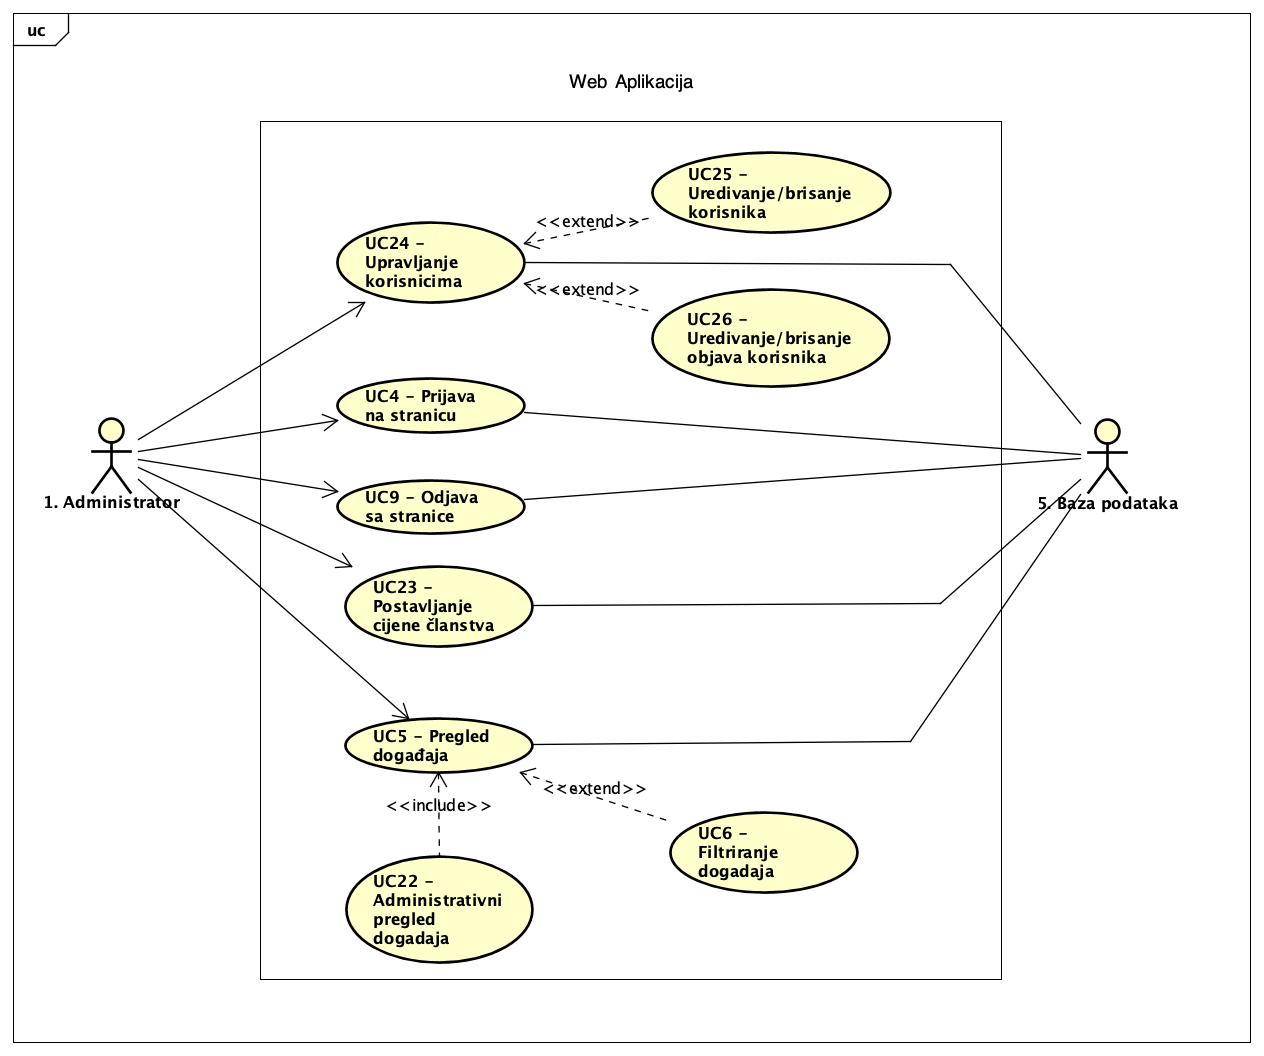
\includegraphics[scale=0.5]{dijagrami/Administrator_UC_dijagram.png} %veličina slike u odnosu na originalnu datoteku i pozicija slike
						\centering
						\caption{Dijagram obrasca uporabe, funkcionalnost administratora}
						\label{fig:promjene}
					\end{figure}
					
					\begin{figure}[H]
						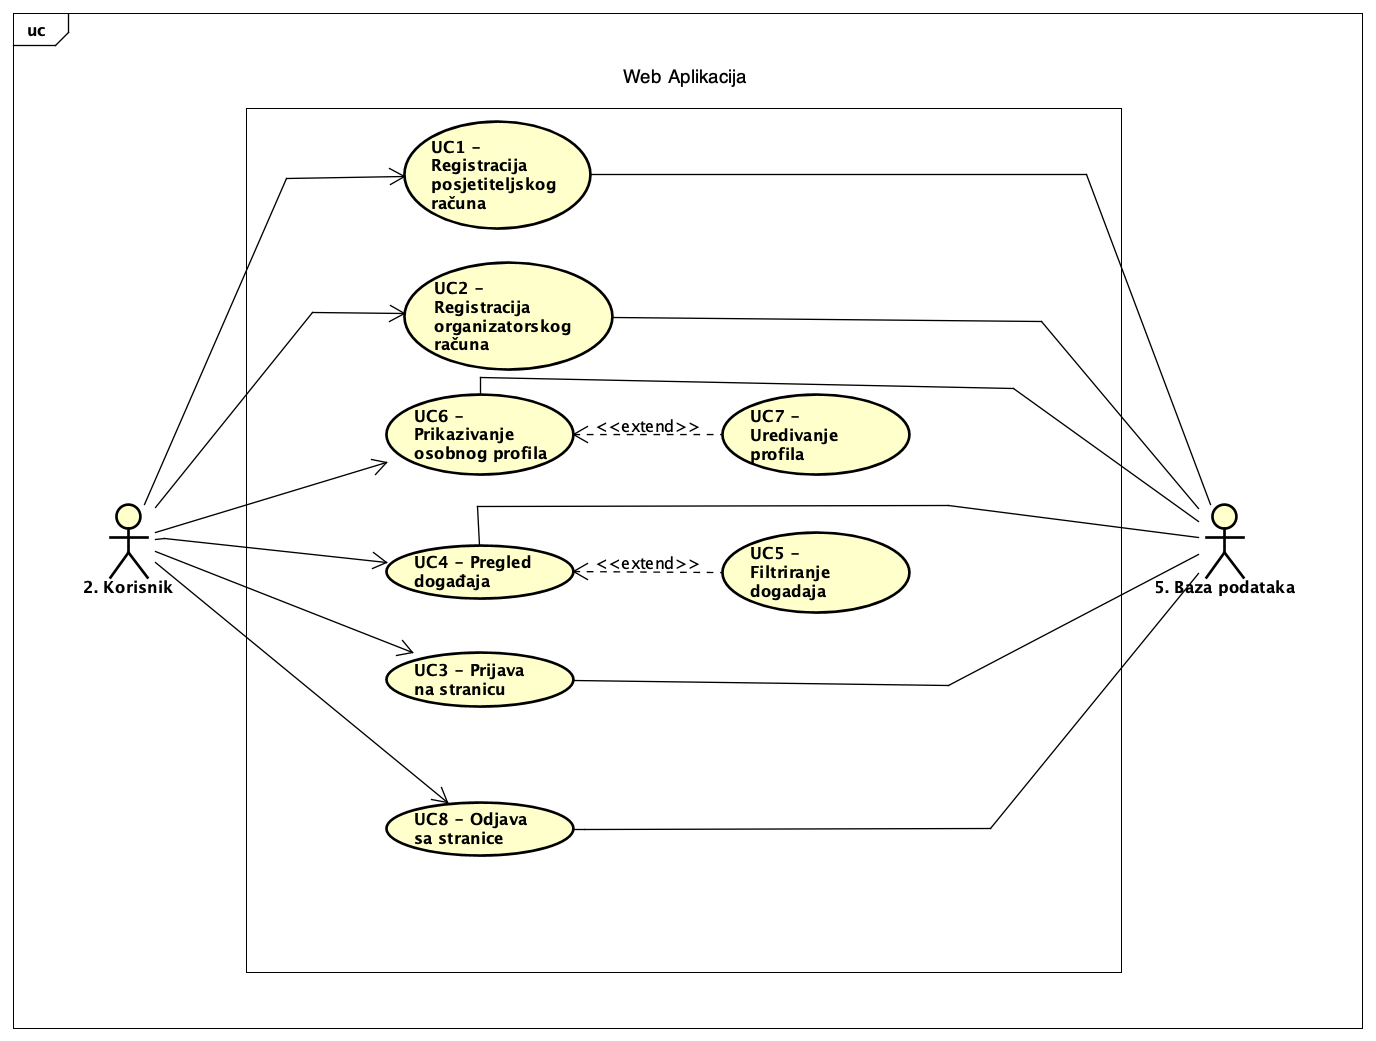
\includegraphics[scale=0.5]{dijagrami/Korisnik_UC_dijagram.png} %veličina slike u odnosu na originalnu datoteku i pozicija slike
						\centering
						\caption{Dijagram obrasca uporabe, funkcionalnost korisnika}
						\label{fig:promjene}
					\end{figure}
					
					\begin{figure}[H]
						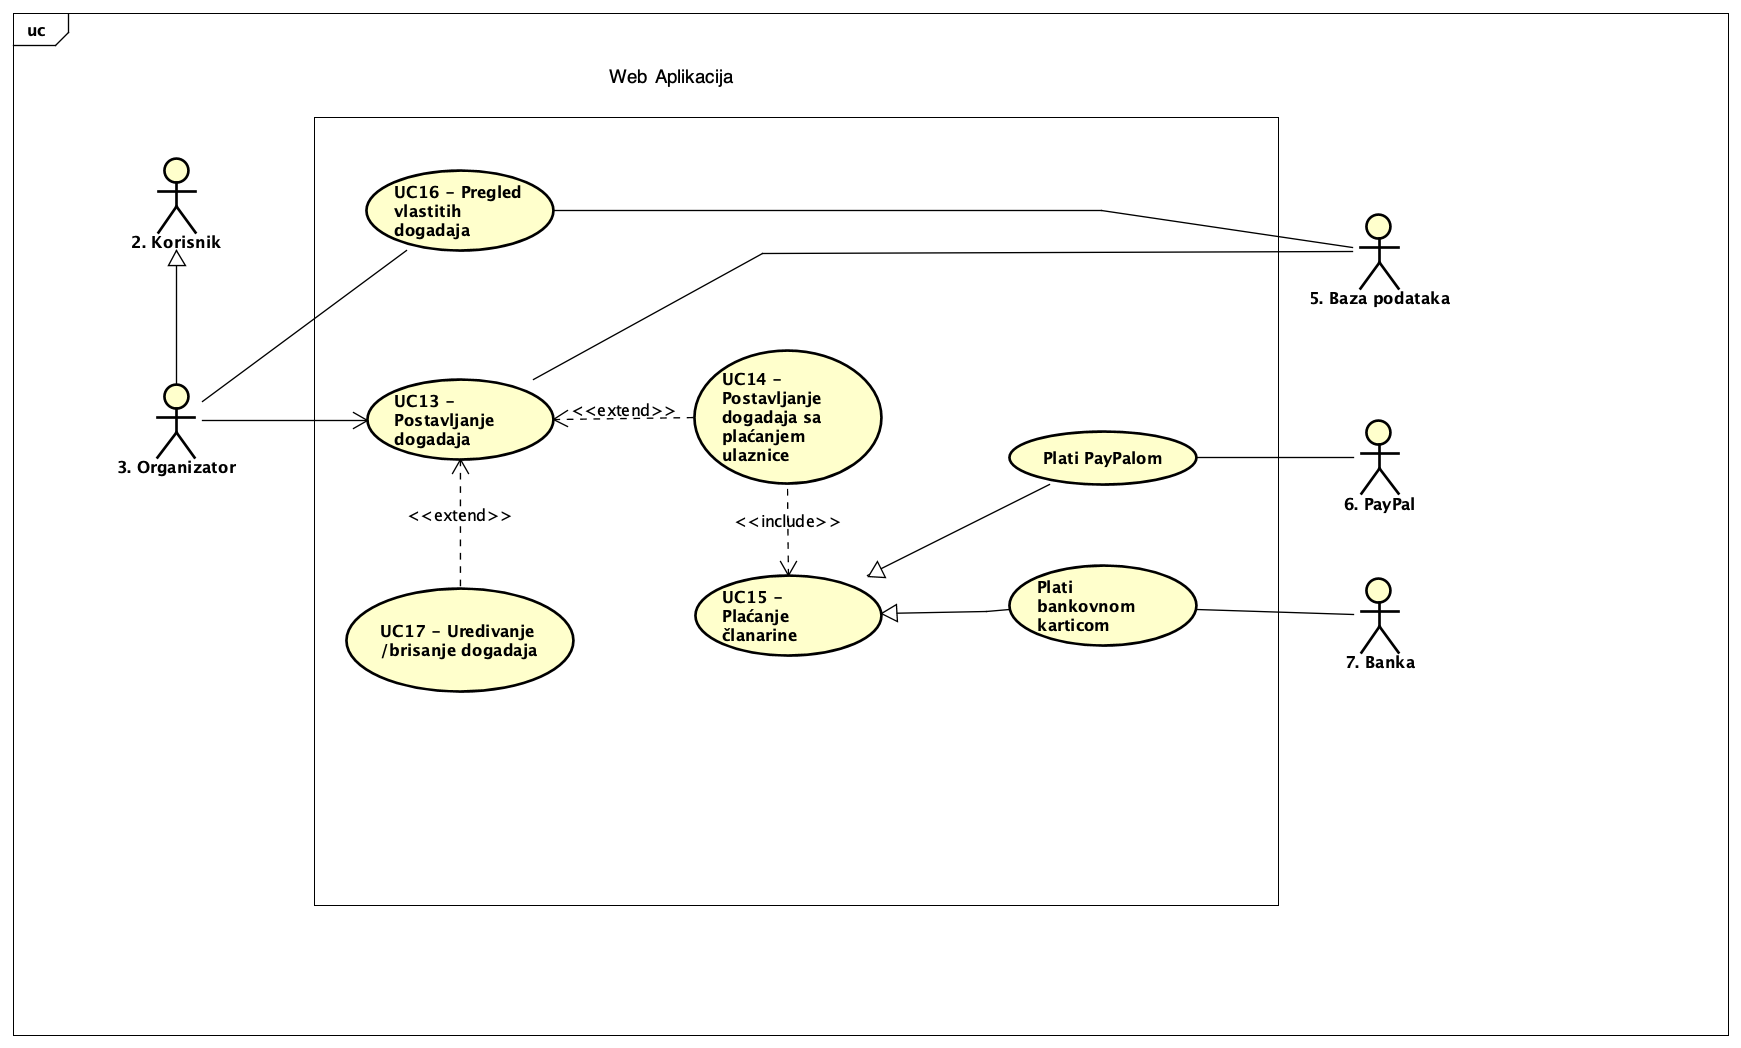
\includegraphics[scale=0.37]{dijagrami/Organizator_UC_dijagram.png} %veličina slike u odnosu na originalnu datoteku i pozicija slike
						\centering
						\caption{Dijagram obrasca uporabe, funkcionalnost organizatora}
						\label{fig:promjene}
					\end{figure}
					
					\begin{figure}[H]
						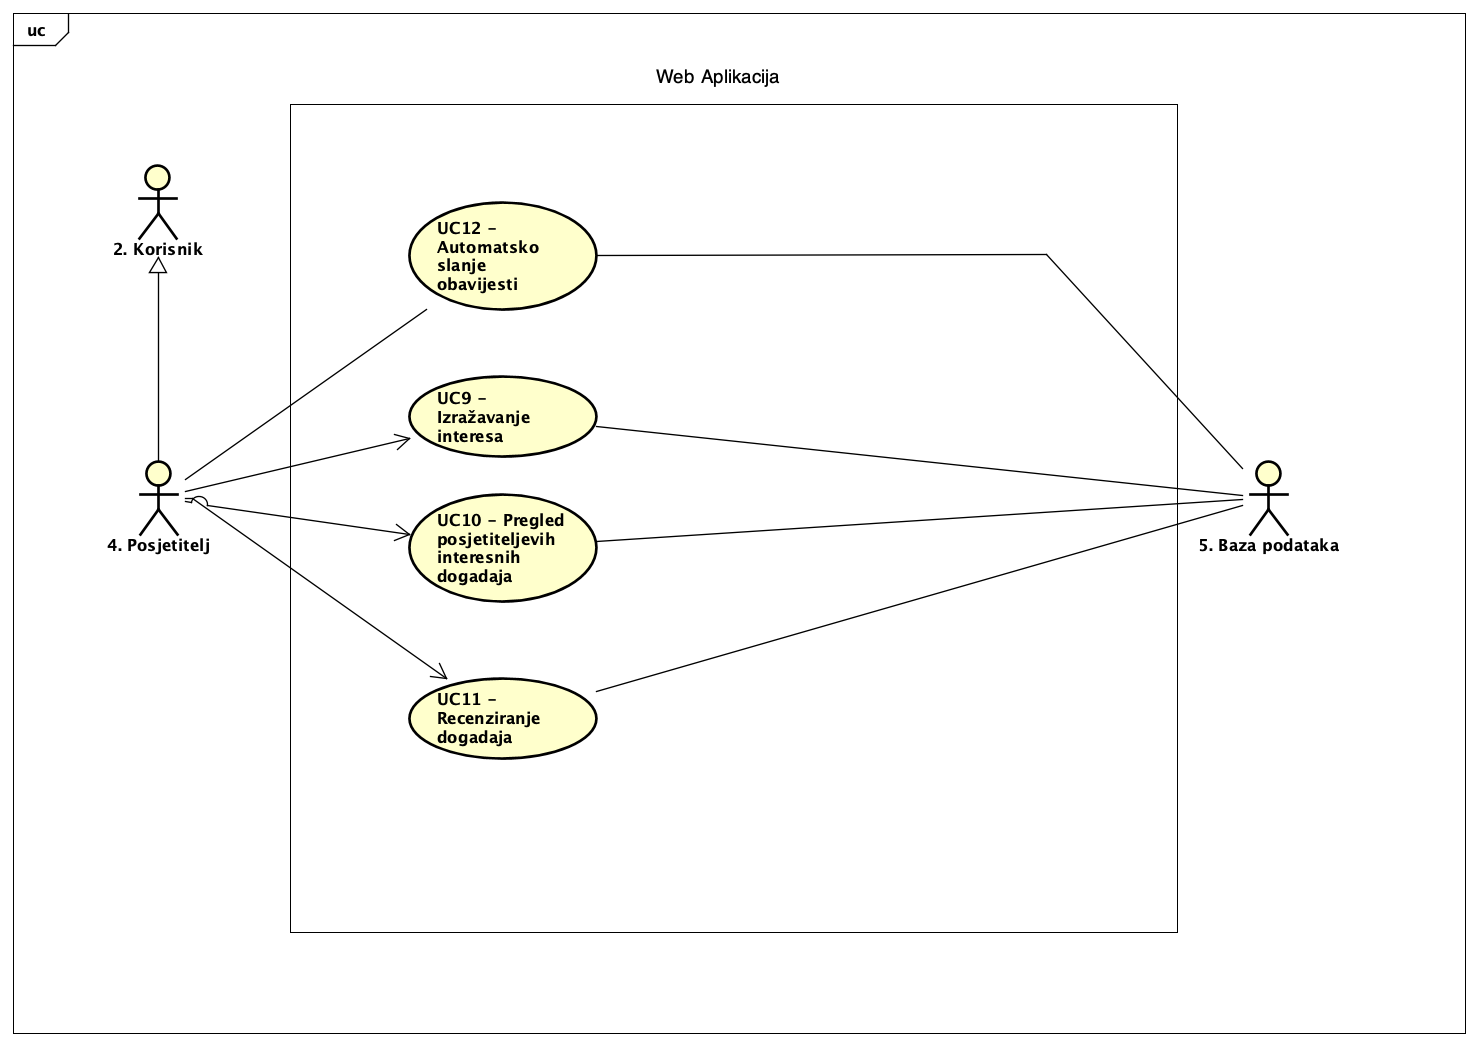
\includegraphics[scale=0.42]{dijagrami/Posjetitelj_UC_dijagram.png} %veličina slike u odnosu na originalnu datoteku i pozicija slike
						\centering
						\caption{Dijagram obrasca uporabe, funkcionalnost posjetitelja}
						\label{fig:promjene}
					\end{figure}
					
				
				\eject		
				
			\subsection{Sekvencijski dijagrami}
				
				\textbf{\textit{dio 1. revizije}}\\
	
				\LARGE {Obrazac uporabe UC1 - Registracija}
				\newline
				\normalsize
				Korisnik prilikom procesa registracije odabire opciju registracije: Posjetitelj ili Organizator. Na temelju odabira, korisnik dohvaća obrazac za registraciju. Nakon ispunjavanja obrasca, korisnik šalje zahtjev za registraciju. Nakon provjere ispravnosti unesenih podataka moguće su dvije opcije:
				
				\begin{packed_item}
					\item {Podaci ispravni:} u slučaju ispravnih podataka vrši se spremanje korisničkih podataka te korisnik prima poruku "Registracija uspješna" te slijedi prikaz za prijavu
					\item {Podaci neispravni:} Korisnik prima poruku da su podaci neispravni te može unijeti podatke ispočetka
				\end{packed_item}
				
				\begin{figure}[H]
					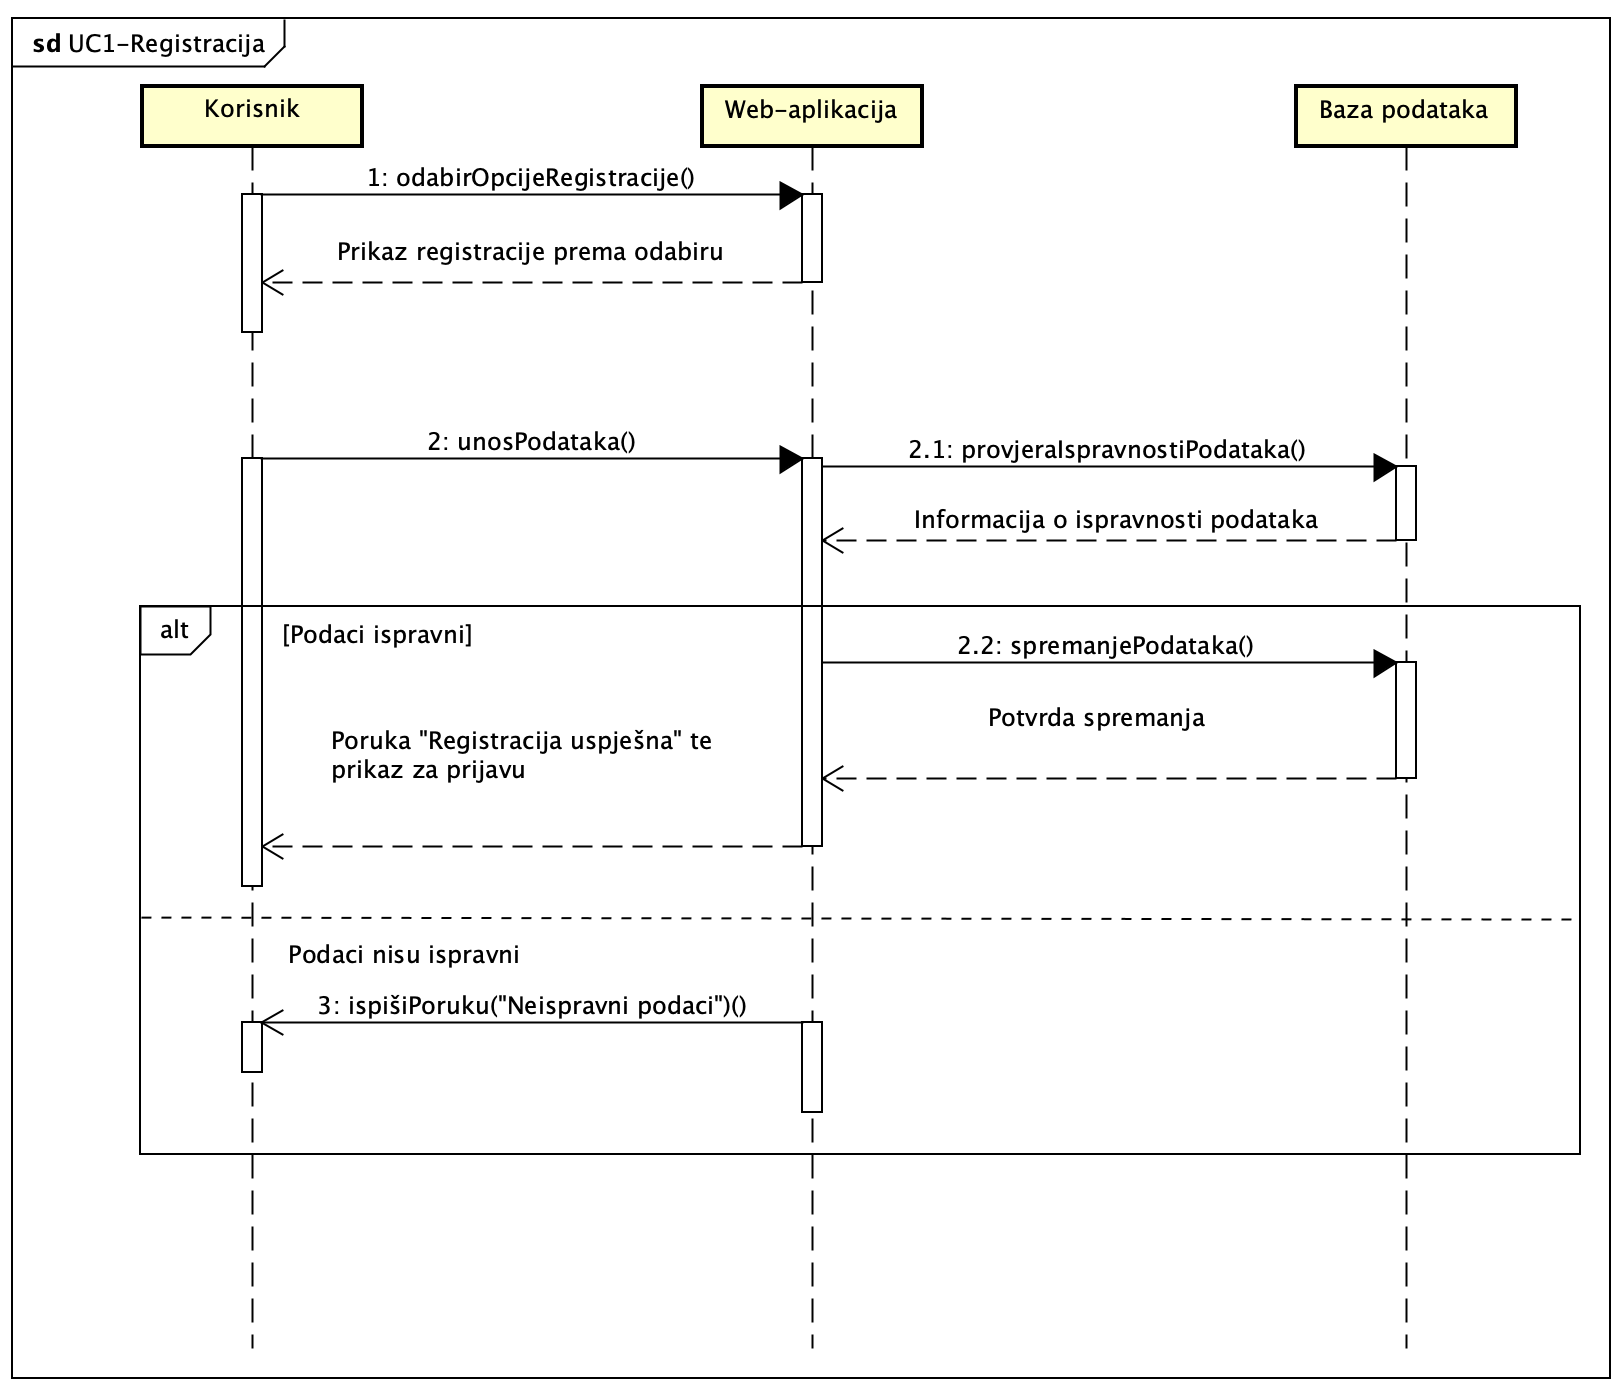
\includegraphics[scale=0.5]{dijagrami/sd-UC1-Registracija.png} %veličina slike u odnosu na originalnu datoteku i pozicija slike
					\centering
					\caption{Sekvencijski dijagram za UC1}
					\label{fig:promjene}
				\end{figure}
				\eject		
				
				\LARGE {Obrazac uporabe UC16 - Postavljanje događaja}
				\newline
				\normalsize
				Tijekom procesa postavljanja događaja Organizator ima mogućnost izabrati objavu bez plaćanje ulaznice za događaj ili uz plaćanje. U slučaju postavljanja događaja bez plaćanja ulaznice odmah dohvaća obrazac za novi događaj. 
				Nakon slanja popunjenog obrasca sa svim potrebnim informacija, Organizator zaprima potvrdu za postavljanje događaja te ima mogućnost potvrditi ili odustati od objave. Ukoliko dođe do potvrde, informacije o događaju se spremaju te se isti objavljuje, u suprotnom Organizator dobiva potvrdu odustajanja.
				
				\begin{figure}[H]
					\includegraphics[scale=0.5]{dijagrami/sd-UC16-Postavljanje-događaja.png} %veličina slike u odnosu na originalnu datoteku i pozicija slike
					\centering
					\caption{Sekvencijski dijagram za UC16}
					\label{fig:promjene}
				\end{figure}
				\eject		
				
				\LARGE {Obrazac uporabe UC19 - Plaćanje članarine}
				\newline
				\normalsize
				Tijekom procesa objave događaja moguće je izabrati opciju za plaćanje ulaznice te u tom slučaju prije slanja obrasca za postavljanje novog događaja dolazi do plaćanje članarine ukoliko je potrebno. 
				Organizator odabire način plaćanje te mu se prikazuje sučelje za unos podataka od izabranog izvora sa trenutnom cijenom članarine. U ovom trenutku Organizator može nastaviti sa procesom plaćanja ili odustati. U slučaju odustajanja dobiva potvrdu, a u suprotnom šalje ispunjen obrazac za plaćanje. Na temeju poslanog obrasca se izvršava plaćanje koje može biti uspješno ili neuspješno. Nakon uspješnog plaćanja se navedene promjene spremaju te Organizator dobiva potvrdu transakcije i novi prikaz. U slučaju neuspješne transakcije Organizator dobiva poruku i razlog neuspješne transakcije.
				
				\begin{figure}[H]
					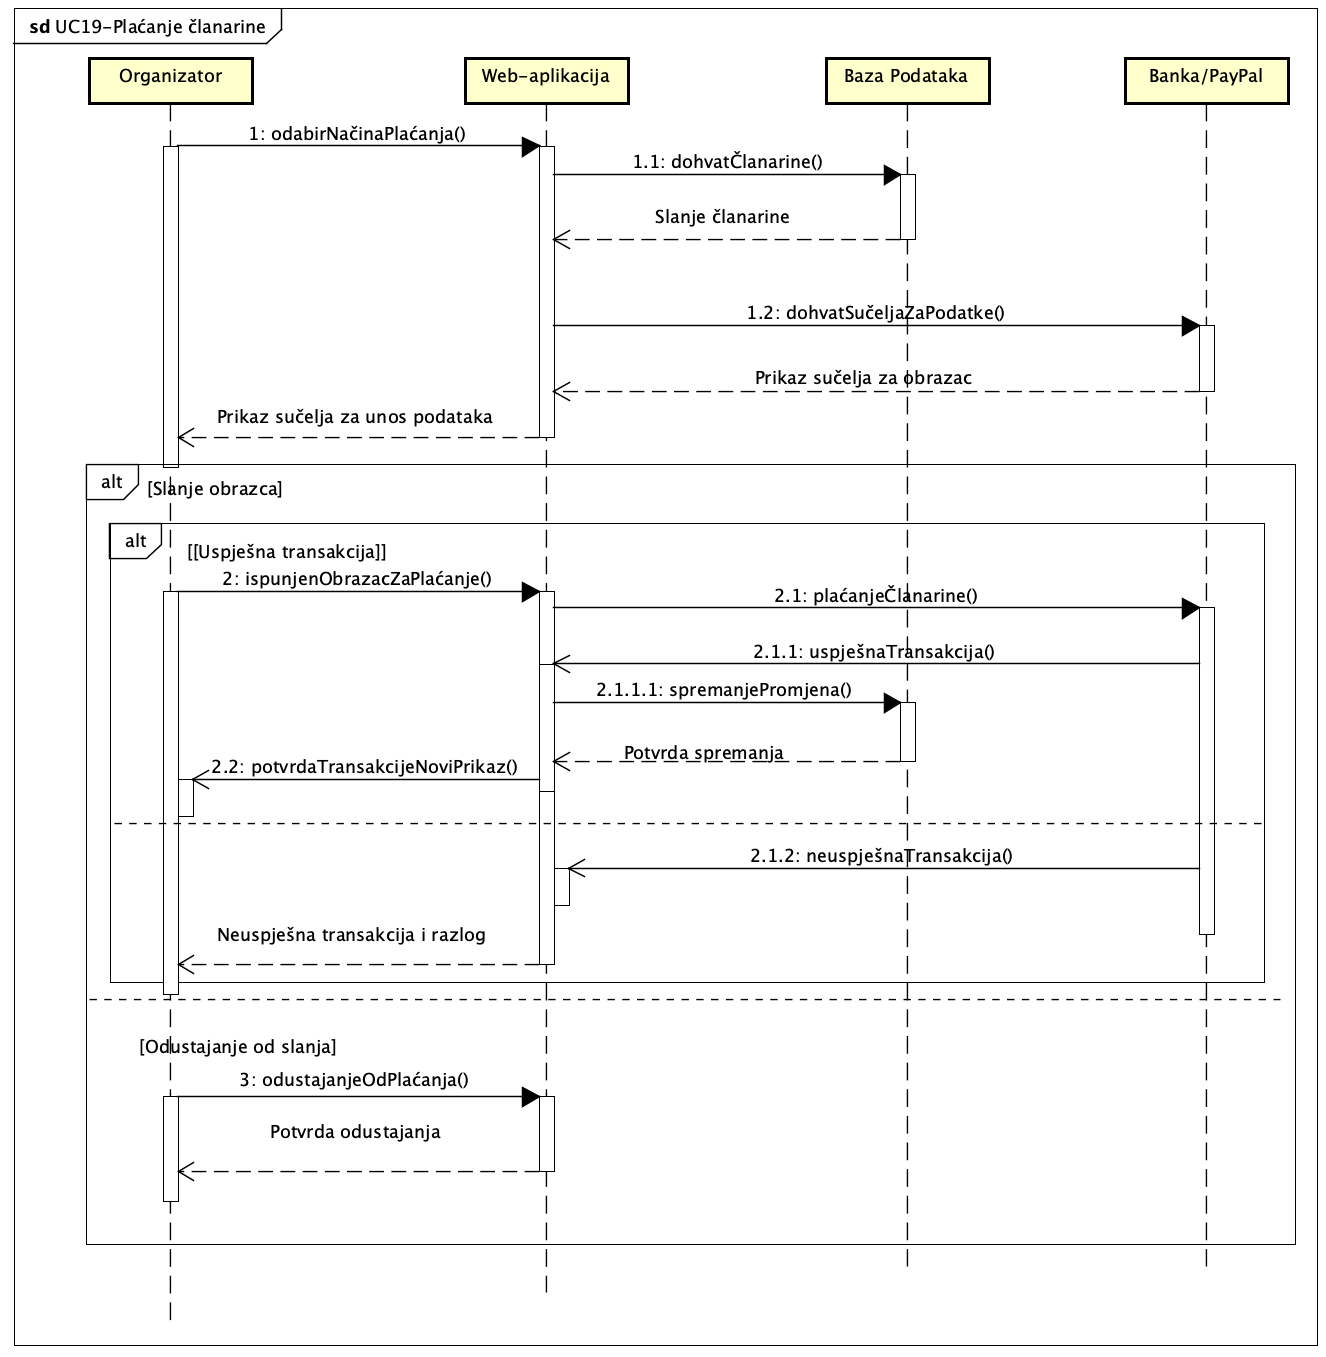
\includegraphics[scale=0.5]{dijagrami/sd-UC19-Placanje-clanarine.png} %veličina slike u odnosu na originalnu datoteku i pozicija slike
					\centering
					\caption{Sekvencijski dijagram za UC19}
					\label{fig:promjene}
				\end{figure}
				\eject		
				
		\section{Ostali zahtjevi}

			 \begin{packed_item}
			\item Sustav treba omogućiti brzo i učinkovito pregledavanje aktualnih događanja, uz minimalno vrijeme odziva aplikacije.
			\item Korisničko sučelje i sustav moraju podržavati različite vrste događanja i inicijativa, prilagođene različitim interesima zajednice.
			\item Izvršavanje dijela programa u kojem se pristupa bazi podataka ne smije trajati duže od nekoliko sekundi kako bi se osigurala brza dostupnost informacija.
			\item Sustav treba biti implementiran kao web-aplikacija koristeći suvremene tehnologije i objektno-orijentirane jezike.
			\item Neispravno korištenje korisničkog sučelja ne smije narušiti funkcionalnost i rad sustava, a sustav treba pružiti jasne upute korisnicima o načinu korištenja.
			\item Sustav treba podržavati različite načine plaćanja članarine, uključujući PayPal i kreditne kartice, te osigurati sigurnost transakcija.
			\item Veza s bazom podataka mora biti kvalitetno zaštićena, brza i otporna na vanjske greške kako bi se očuvala integritet podataka.
			\item Pristup sustavu mora biti omogućen iz javne mreže pomoću HTTPS kako bi se osigurala sigurna komunikacija između korisnika i sustava.
			\item Administratori sustava trebaju imati alate za postavljanje cijena članstva, upravljanje korisnicima i održavanje cjelokupnog sustava.
			 \end{packed_item}
			 
			 
	